\slajdid{09_3-s047}
\begin{frame}[label=09_3-s047]{NMOS izlaz sa otvorenim drejnom}
% element: 09_3-s047:e01
% element: 09_3-s047:e02
% element: 09_3-s047:e03
% element: 09_3-s047:e04
PUN dodaje korisnik, najčešće otpornikom.\begin{columns}[c,onlytextwidth]\column{.25\textwidth}\centering{\RazaviSetup
\ctikzset{transistors/scale=.60}\begin{tikzpicture}[line width=.7pt,x=.65cm,y=.65cm,font=\sitneoznake]\begin{scope}[shift={(0,0)}]\node[rz nmos,nobulk,anchor=D] (M1) at (.4,.65) {};\draw[wire](M1.S)--(.4,-.65);\draw[wire](-1,0)node[left]{A} -| (M1.G);\end{scope}\node[right]at(.55,0){N};\draw(.4,.65)--(.4,1.1)--(.9,1.1)node[ocirc]{}node[right]{Y};\draw(.4,-.65)--(.4,-1.0)node[ground]{};\end{tikzpicture}

}
\par\medskip\begin{tabular}{c|c}A&Y\\\hline0&Z\\1&0\end{tabular}\column{.41\textwidth}\begin{center}
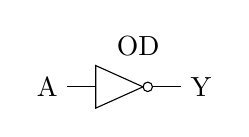
\begin{tikzpicture}[x=.6cm,y=.6cm,font=\sitneoznake]
\draw(0,-.45)--(1,0)--(0,.45)--cycle;\draw(1.1,0)circle(.1);\draw(-.6,0)node[left]{A}--(0,0);\draw(1.2,0)--(1.8,0)node[right]{Y};\node[above]at(.9,.45){OD};\end{tikzpicture}

\end{center}\begin{itemize}
\item \alert{Izlaze smemo povezati.}
\item Zakočen N → visoka impedansa.
\item $Z$ nije vrednost Bulove algebre.
\item Plutajući ulazi reaguju na smetnje.
\end{itemize}\column{.30\textwidth}\centering\begin{tikzpicture}[x=.7cm,y=.6cm,font=\sitneoznake,>=Latex]
\draw(0,.25)--(0,.75);\draw(-.13,.22)--(-.13,.78);\draw(0,.7)--(.4,.7)--(.4,1.1);\draw(0,.3)--(.4,.3)--(.4,-.35)node[ground]{};
\draw(-.75,.5)--(-.13,.5);\draw(-1.15,1.15)node[ocirc]{}node[left]{$V_I$}--(-.75,1.15);\node[right]at(.55,.5){N};
\draw(0,1.65)--(0,2.15);\draw(-.13,1.62)--(-.13,2.18);\draw(0,2.1)--(.4,2.1)--(.4,2.65);\draw(0,1.7)--(.4,1.7)--(.4,1.1);
\draw(-.22,1.9)circle(.09);\draw(-.31,1.9)--(-.75,1.9)--(-.75,.5);\node[right]at(.55,1.9){P};
\draw(.15,2.65)--(.65,2.65)node[above left]{$V_{DD}$};\draw(.4,1.15)--(1.1,1.15)node[ocirc]{}node[right]{$V_O$};
\end{tikzpicture}


\end{columns}
\end{frame}
